\documentclass[10pt,preprint]{article}
\usepackage[latin1]{inputenc}
\usepackage{amsmath}
\usepackage{amsfonts}
\usepackage{amssymb}
\usepackage{mathtools}
\usepackage{fullpage}

\newcommand{\pt}{\propto}
\newcommand{\rp}{\right)}
\newcommand{\lp}{\left(}

\begin{document}

\begin{center}
\textbf{\begin{huge} September 6, 2011\end{huge}}\\
\begin{large}Jeren Suzuki\end{large}
\end{center}

\section{Energy Transport by Radiation (\& Conduction)}
So in the beginning...\\
\\

\section{Energy Transport by Conduction}
\begin{figure}[!ht]
\centering
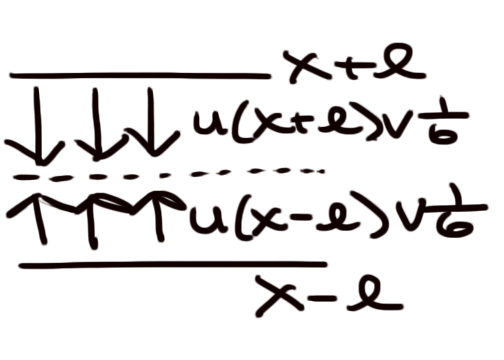
\includegraphics[width=\textwidth /2]{9-6/fig1.png}
\label{fig:1}
\end{figure}

Figure \ref{fig:1} shows the stratification levels of the inside of a star at a given height $x$ with a length $l$  either up or down. \\
\begin{list}{}{}
\item $T$ = temp
\item $u$ = Thermal Energy Density
\item $v$ = velocity
\item $l $= mean free path
\end{list}

The factor of $\frac{1}{6}$ is used because we multiply $\frac{1}{3}$ (from 3 degrees of translational freedom) with $\frac{1}{2}$ (from going up and down).

\begin{align*}
F \equiv ~\text{net flux of energy} = \frac{1}{6}u(x-l)v - \frac{1}{6}u(x+l)v
\end{align}
Taylor expanding $u(x-l) = u(x) - \frac{du}{dx}l$, we get:

\begin{align*}
F = -\frac{1}{3}vl\frac{du}{dx}~,~\text{or more generally,}~F=-\chi \nabla u
\end{align}

For a gas of charged particles,

\begin{align*}
U &= n\frac{3}{2}kT\\
F &= -\frac{1}{3}vl \frac{dU}{dT}\frac{dT}{dx}~,~\text{where}~\frac{dU}{dT}~\text{is the specific heat}.\\
\Aboxed{F &= -\frac{1}{2}vlnk \frac{dT}{dx}}
\end{align}

In the case of a charged particle moving past another charged particle, there is a characterized distance ($b$) where the change in trajectory is significant. 

\begin{align*}
\frac{q^2}{b} &\sim kT\\
b &\sim \frac{q^2}{kT}\\
\text{effective area }=\sigma &= \pi b^2\\
\Aboxed{\sigma &= \frac{\pi q^4}{(kT)^2}}
\end{align*}

\begin{align*}
F &=-\frac{1}{2}nklv\frac{dT}{dx}~,v \sim v_{thm} = \sqrt{\frac{kT}{m}}\\
&\sim -\frac{1}{2} \frac{kv}{\sigma}\frac{dT}{dx}\\
&=-\chi \frac{dT}{dx}~,\text{where }\chi =\frac{1}{2}\frac{kv}{\sigma} \pt \frac{T^{5/2}}{\sqrt{m}}
\end{align}

Electrons move faster than protons so they transfer energy much more effectively. Electrons and protons have the same $\sigma$, but the difference in velocities is huge.

\subsection{How important is this energy transport in the sun?}

\begin{align*}
F &= -\chi \frac{dT}{dx}\\
L &= 4 \pi r^2 F\\
&\sim 4 \pi R^2 \chi \frac{T_c}{R}~\text{(We're doing a poor man's derivative where $\frac{dT}{dx} = \frac{T_c}{R}$)}\\
L &\sim \frac{k^{7/2} T_c^{7/2} R}{q^4 \ln (\Lambda) \sqrt{m_e}}\\
&\sim 10^{-4} L_\odot \lp \frac{R}{R_\odot} \rp \lp \frac{T_c}{10^7\text{ K} } \rp^{7/2}
\end{align*}

Doing this, we get that $L_{conduction} \ll L_\odot$ and therefore electron conduction is unimportant to energy transport. 

\section{Radiation Transport of Energy}
\begin{list}{}{}
\item $U = aT^4$
\item $l = \frac{1}{n \sigma}$
\item $\sigma$ = cross section for photons to interact with matter, not with other photons
\end{list}

\begin{align*}
F &=-\frac{1}{3}cl \frac{d}{dr}aT^4\\
&= -\frac{4}{3}claT^3 \frac{dT}{dr}\\
\Aboxed{&=-\frac{4}{3}\frac{caT^3}{\kappa \rho} \frac{dT}{dr}}
\end{align}

For an Ionized plasma with dominant photon-matter interactions through electron scattering (Thomson Scattering),

\begin{align*}
m_e \bar{a} &= -e(\bar{E} + \frac{\bar{v}}{c} \times \bar{B})\\
|E| &= |B|\\
m_e\bar{a} &= -e\bar{E}\text{ since $ \frac{\bar{v}}{c} \times \bar{B}$ is small}\\
\bar{a} &= -\frac{e \bar{E}}{m_e}
\end{align}

\begin{align*}
P &= \frac{2}{3}\frac{e^4}{c^3 m_e^2}|\bar{E}|^2\\
\sigma F &= P\\
\sigma \frac{c}{4\pi}|\bar{E}| &= \frac{2}{3}\frac{e^4}{c^3 m_e^2}|\bar{E}|^2\\
\Aboxed{\sigma_T &= \frac{8\pi}{3}\frac{e^4}{m_e^2 c^4} = \text{ Thomson cross-section or $e^-$-scattering cross-section}}
\end{align}

\begin{align*}
\sigma_T &= \frac{8\pi}{3}r_c^2,~\text{ where $r_c$ is the classical radius of the $e^-$}\\
r_c &=\frac{e^2}{m_e c^2} \approx 2.8 \times 10^{-13} \text{ cm},
\end{align}
which should strike as odd since $e^-$ has no observed structure but still has an "effective radius".

\end{document}